\section{Проектирование реализации и описание программной системы}


\begin{figure}[h]
    \centering
    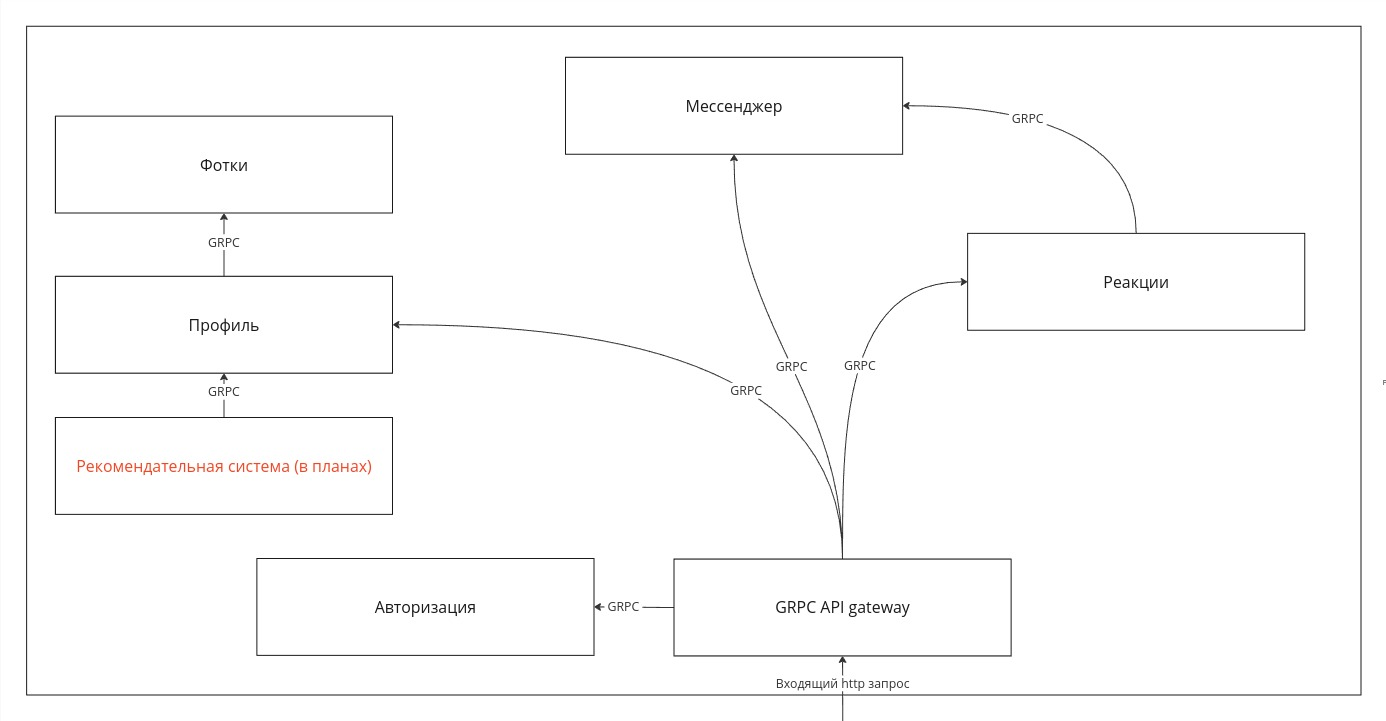
\includegraphics[width=1\columnwidth ]{glimpse - Схема межсервисного взаимодействия.jpg}
    \caption{Схема межсервисного взаимодействия}
\end{figure}

В данном разделе рассмотрим проектирование реализации нашего приложения для знакомств, основанного на микросервисной архитектуре. Схема межсервисного взаимодействия представлена на рисунке и описывает, как различные компоненты приложения взаимодействуют друг с другом посредством \textbf{gRPC}.

\textbf{Основные компоненты системы:}

\begin{itemize}
    \item \textbf{GRPC API Gateway:} Этот компонент служит центральной точкой входа для всех HTTP-запросов, поступающих в систему. API Gateway принимает запросы от клиентов и маршрутизирует их к соответствующим микросервисам, используя gRPC. Это обеспечивает единый интерфейс для внешних взаимодействий и упрощает управление трафиком.
    
    \item \textbf{Авторизация:} Микросервис, отвечающий за аутентификацию и регистрацию пользователей. Он обрабатывает запросы на вход в систему, проверяет учетные данные пользователей и выдает токены доступа, которые используются для последующих запросов через API Gateway.
    
    \item \textbf{Профиль:} Микросервис, управляющий профилями пользователей. Он обрабатывает запросы на создание, редактирование и удаление профилей, а также хранит и предоставляет данные профилей другим микросервисам по gRPC.
    
    \item \textbf{Фотки:} Этот микросервис отвечает за загрузку и хранение фотографий пользователей. Он взаимодействует с микросервисом профилей для привязки фотографий к соответствующим профилям пользователей.
    
    \item \textbf{Мессенджер:} Микросервис для обмена сообщениями между пользователями. Использует ScyllaDB для хранения сообщений и обеспечивает возможность отправки и получения текстовых и голосовых сообщений.
    
    \item \textbf{Реакции:} Микросервис, который управляет реакциями пользователей на профили других пользователей. Он обрабатывает лайки, дизлайки и другие виды реакций, а также предоставляет данные о реакциях другим компонентам системы.
    
    \item \textbf{Рекомендательная система (в планах):} Будет разработана для предоставления пользователям персонализированных рекомендаций на основе их профилей и поведения в приложении. Этот микросервис будет взаимодействовать с профилем и реакциями для получения необходимых данных.
\end{itemize}

\textbf{Межсервисное взаимодействие:}

Все микросервисы взаимодействуют друг с другом с помощью gRPC, что обеспечивает высокую производительность и низкую задержку при обмене данными. Основные потоки данных и взаимодействия между микросервисами включают:

\begin{itemize}
    \item API Gateway принимает входящие HTTP-запросы от клиентов и маршрутизирует их к соответствующим микросервисам через gRPC.
    \item Микросервис Авторизации взаимодействует с API Gateway для аутентификации пользователей и выдачи токенов доступа.
    \item Микросервис Профилей взаимодействует с Фотками для управления фотографиями пользователей и с Реакциями для обработки реакций на профили.
    \item Мессенджер взаимодействует с Реакциями и Профилями для обеспечения контекста сообщений и управления диалогами.
    \item В перспективе, Рекомендательная система будет интегрирована с Профилями и Реакциями для предоставления персонализированных рекомендаций пользователям.
\end{itemize}

Такое проектирование обеспечивает модульность, масштабируемость и гибкость системы, что позволяет легко добавлять новые функции и улучшать существующие компоненты без значительных изменений в архитектуре приложения.
